\section{Time-Step Averages of White Noise with Varying Sample Size}

We seek to take the ARMA-Noise model and generalize it to allow for $\{n_t\}$ to vary, as is so often the case in real RCS survey data. We will now treat $\{n_t\}$ as the realizations of random variables $\{N_t\}_{t=1}^T$. What we aim to establish are the conditions under which the random variable $A_t = N_t^{-1}\sum_{i=1}^{N_t}\varepsilon_{ti}$ is still white noise.

First, let $\{N_t\}$ be i.i.d. random variables with a sample space that is a subset of the integers strictly greater than $0$. The conditional random variable $A_t|N_t$ then has variance $\sigma_\varepsilon^2/N_t$. However, note that this is the variance of $A_t$ after being conditioned on $N_t$, not its marginal variance. 

To find Var($A$) we use the Law of Total Variation:

\begin{equation}
    \label{eq:totalvar}
    \text{Var}(A) = \mathbb{E}(\text{Var}(A|N)) + \text{Var}(\mathbb{E}(A|N))
\end{equation}

Now, Var$(A|N) = \sigma_\varepsilon^2N^{-1}$, and therefore has an expectation of $\sigma_\varepsilon^2\mathbb{E}(N^{-1})$. At the same time, the expectation of $A$ is $0$ regardless of the value of $N$, meaning the second term in Equation \ref{eq:totalvar} is zero, leaving only Var$(A) = \sigma_\varepsilon^2\mathbb{E}(N^{-1})$. It's worth identifying at this time the conditions under which $\mathbb{E}(N^{-1})$ is defined, but this will always be the case (so long as $N \geq 1$ a.s.).

Proof:

$$ N \geq 1 \qquad \text{a.s.} $$

$$ \Rightarrow0 < N^{-1} \leq 1 \qquad \text{a.s.}  $$

$$ \Rightarrow 0 < \mathbb{E}(N^{-1}) \leq 1 \qquad \text{a.s.}  $$


Now, it is worth noting that $A$ is only Gaussian if $\{n_t\}$ is almost surely constant. However, our claim is that $\{a_t\}$ is still white noise, just with variance $\sigma_\varepsilon^2\mathbb{E}(N^{-1})$. To establish this, we must show that it is a zero-mean stationary process with ACVF $\gamma_A(h) = \mathbbm{1}_{\{0\}}(h)\sigma^2$.

Firstly, we can quickly verify that $A_t$ is zero mean with the Law of Total Expectation:
$$ \mathbb{E}(A_t) = \mathbb{E}(\mathbb{E}(A_t|N_t)) = \mathbb{E}(0) = 0 $$

Now we've already established $\text{Var}(A_t)$ to be independent of $t$, so we now verify that $\text{Cov}(A_r,A_s) = 0$ for $r \neq s$. The Law of Total Covariance states:


$$ \text{Cov}(A_r,A_s) = \mathbb{E}(\text{Cov}(A_r,A_s|N_r,N_s)) + \text{Cov}(\mathbb{E}(A_r|N_r), \mathbb{E}(A_s|N_s))$$

Given that $A_r$ and $A_s$ are functions of independent random vectors $\bm{\varepsilon}_r \in \mathbb{R}^{n_r}$ and $\bm{\varepsilon}_s \in \mathbb{R}^{n_s}$, $\text{Cov}(A_r,A_s|N_r,N_s)$ must be zero. Having already established that both variables are zero-mean, the above equation reduces to:

$$ \text{Cov}(A_r,A_s) = \mathbb{E}(0) + \text{Cov}(0, 0) = 0$$

Having shown that $\{A_t\}$ is still white noise, it now remains to estimate its variance. Though the sample sizes now vary, our estimate for $\sigma_\varepsilon^2$ hasn't changed:

\begin{equation}
    \hat{\sigma}_\varepsilon^2 =(N-T)^{-1}\sum_{t=1}^T\sum_{i=1}^{n_t}(w_{ti}-\bar{w}_{t\cdot})^2 
    \label{eq:var_eps_hat}
\end{equation}
Without requiring the distribution of $N_t$, $\sigma_a^2$ can be estimated with:

\begin{equation}
    \label{eq:var_a_n}
    \hat{\sigma}_a^2 = \frac{\hat{\sigma}_\varepsilon^2}{T}\sum_{t=1}^T\frac{1}{N_t}
\end{equation}


While we're still maintaining the independence of $N_t$, it's worth noting that at no point in the above reasoning was such a characteristic used in establishing $A_t$ as white noise. Before exploring the implications of such an observation, let's look at some sample distributions for $N_t$ that show the importance of using this estimator as opposed to more naive ones.


\textbf{Example:} $N_t \overset{d}{=} M_t + 1, \qquad M_t \sim \text{Poi}(\lambda)$ 

$N_t \geq 1, \text{ a.s.}$ so we know that $\mathbb{E}(N_t^{-1})$ exists. We derive it now:

$$   \mathbb{E}(N^{-1}) = \sum_{n=0}^\infty \frac{e^{-\lambda}\lambda^n}{n!(n+1)} =  \frac{1}{\lambda}\sum_{n=0}^\infty \frac{e^{-\lambda}\lambda^{n+1}}{n!(n+1)} = \frac{1}{\lambda}\sum_{n=0}^\infty \frac{e^{-\lambda}\lambda^{n+1}}{(n+1)!} = \frac{1}{\lambda}(1-e^{-\lambda})  $$

From this we obtain the following expression for the variance of $a_t$:
\begin{equation}
    \label{eq:var_a_poi}
    \text{Var}(a_t) = \frac{\sigma_\varepsilon^2(1-e^{-\lambda})}{\lambda}
\end{equation}



We can validate this through simulating i.i.d. samples of $N_t = M_t + 1$, with  $M_t \overset{\text{i.i.d.}}{\sim}\text{Poi}(\lambda)$, then for each value of $t=1,...,T$ we simulate $N_t$ i.i.d. realizations of Gaussian noise $\varepsilon_{ti}$ with variance $\sigma_\varepsilon^2$. We set $\lambda = 2$, $\sigma_\varepsilon^2 = 10$,  and $T = 1,000,000$. 


Equation \ref{eq:var_a_poi} yields a value of roughly $\sigma_a^2 = 4.323$ with the given parameters.
Given these are simulated data, we have explicit observations of the vector $\mathbf{a}$, a luxury we won't have when fitting estimates to $X_t\uu + \bm{\varepsilon}$. 

The set $\{a_t\}$ had a sample variance of $4.324$. Turning to our estimates, Equation \ref{eq:var_a_poi} produced an estimate $\hat{\sigma}_a^2 \approx 4.323$, while naively estimating $\sigma_a^2$ by dividing $\hat{\sigma}_\varepsilon^2$ by the mean sample size resulted in the estimate $\frac{\hat{\sigma}_\varepsilon^2}{\bar{n}}=3.332$. This disparity highlights the need for the estimator defined above.

% \textcolor{blue}{$\widehat{\sigma_a^2}$ appeared to beat $S_a^2$ every time...coincidence?}. 

% Example: $N_t \sim \text{Bin}(n,p) + 1 $:

% $$ \mathbb{E}(N_t) = np + 1 $$

% $$ \mathbb{E}(N_t^{-1}) = \sum_{x = 0}^n \left( \begin{array}{c}
%      n \\
%      x
% \end{array} \right) p^x (1 - p)^{n-x}(x+1)^{-1} = \sum_{x = 0}^n \frac{n!}{(x+1)!(n-x)!}p^x(1-p)^{n-x} $$

% $$ \mathbb{E}(N_t^{-1}) = (n+1)^{-1}p^{-1}\sum_{x = 0}^n \frac{(n+1)!}{(x+1)!(n-x)!}p^{x+1}(1-p)^{n-x} = \frac{1 - (1-p)^{n + 1}}{(n+1)p} $$
Now that we have an estimate for $\sigma_a^2$, let's see how this change in estimator affects the rest of the method.

\section{ARMA-Noise Models with I.I.D. Sample Size}


When sample sizes are allowed to vary over time, an ARMA-Noise model changes:

$$ w_{ti} = u_t + \varepsilon_{ti}, \qquad \{u_t\} \sim \text{ARMA}(\phi,\theta,\sigma_\eta^2,T), \qquad \varepsilon_{ti}\overset{\text{i.i.d.}}{\sim}N(0,\sigma_\varepsilon^2)$$

$$ \bar{w}_{ti} = n_t^{-1}\sum_{i = 1}^{n_t}w_{ti} =  u_t + a_t, \qquad a_t = n_t^{-1}\sum_{i=1}^{n_t}\varepsilon_{ti}$$

$$ \{n_t\} \text{ are i.i.d.} \qquad \Omega(N) \subseteq \left\{\mathbb{Z}>0\right\} $$

The individual noise variance $\sigma_\varepsilon^2$ is estimated with \ref{eq:var_eps_hat}. We review the variance of this estimate for the purposes of estimating $\Sigma_o$ (Equation \ref{eq:Sigma_o}) 

$$ \text{Var}(\hat{\sigma}_\varepsilon^2) = \text{Var}\left[(N-T)^{-1}\sum_{t\in T_2}(n_t-1)S_t^2\right] $$

Note that we cannot treat $(N-T)$ as a constant as we could with a fixed sample size. We leverage the Law of Total Variance to decompose the variance:
\begin{equation}
    \text{Var} (\hat{\sigma}_\varepsilon^2) = \mathbb{E}(\text{Var}(\hat{\sigma}_\varepsilon^2|\{N_t\})) + \text{Var}(\mathbb{E}(\hat{\sigma}_\varepsilon^2|\{N_t\})) 
    \label{eq:total_var_eps}
\end{equation}


Focusing on the first term in Equation \ref{eq:total_var_eps}, we have: 

$$ \mathbb{E}(\text{Var}(\hat{\sigma}_\varepsilon^2|\{N_t\})) = \mathbb{E}\left(\text{Var}\left[(N-T)^{-1}\sum_{t=1}^T\sum_{i=1}^{n_t}(w_{ti}-\bar{w}_{t\cdot})^2|\{N_t\}\right]\right) $$

Having conditioned on $\{N_t\}$ we obtain the following:

$$ \mathbb{E}(\text{Var}(\hat{\sigma}_\varepsilon^2|\{N_t\})) = \mathbb{E}\left((N-T)^{-2}\text{Var}\left[\sum_{t=1}^T\sum_{i=1}^{n_t}(w_{ti}-\bar{w}_{t\cdot})^2\right]\right) $$

Because of the independence within the set $\{S_t^2\}$ we get:

$$ \mathbb{E}(\text{Var}(\hat{\sigma}_\varepsilon^2|\{N_t\})) = \mathbb{E}\left((N-T)^{-2}\sum_{t=1}^T\text{Var}\left[\sum_{i=1}^{n_t}(w_{ti}-\bar{w}_{t\cdot})^2\right]\right) $$

Having previously derived the variance of $S_t^2$ we arrive at:

$$ \mathbb{E}(\text{Var}(\hat{\sigma}_\varepsilon^2|\{N_t\})) = \mathbb{E}\left((N-T)^{-2}\sum_{t=1}^T2(n_t-1)\sigma^4\right) = 2\sigma^4\mathbb{E}(N-T)^{-1} $$

Let's now turn to the second term:

$$ \text{Var}(\mathbb{E}(\hat{\sigma}_\varepsilon^2|\{N_t\})) = \text{Var}(\mathbb{E}((N-T)^{-1}\sum_{t=1}^T\sum_{i=1}^{n_t}(w_{ti} - \bar{w}_{t\cdot})^2|\{N_t\})) $$

Conditioning on $\{N_t\}$, we can pass the expectation inside the first sum:

$$ \text{Var}(\hat{\sigma}_\varepsilon^2|\{N_t\})) = \text{Var}\left[(N-T)^{-1}\sum_{t=1}^T\mathbb{E}\left(\sum_{i=1}^{n_t}(w_{ti} - \bar{w}_{t\cdot})^2\right)\right] $$

With $(n_t-1)S_t^2$ having expectation $(n_t-1)\sigma_\varepsilon^2$, we arrive at:

$$ \text{Var}(\mathbb{E}(\hat{\sigma}_\varepsilon^2|\{N_t\})) = \text{Var}((N-T)^{-1}\sum_{t}(n_t-1)\sigma_\varepsilon^2) $$
We can then pull out the $\sigma_\varepsilon^2$:

$$ \text{Var}(\mathbb{E}(\hat{\sigma}_\varepsilon^2|\{N_t\})) = \sigma_\varepsilon^4\text{Var}((N-T)^{-1}(N-T)) = 0 $$

This is consistent with the fact that, whatever $\{N_t\}$ is, $\hat{\sigma}_\varepsilon^2$ is unbiased for $\sigma_\varepsilon^2$, therefore having no variance. We're therefore left with:

$$ \text{Var}(\hat{\sigma}_\varepsilon^2) = 2\sigma^4\mathbb{E}(N-T)^{-1} $$
With only one set of sample sizes, our only estimate for $\mathbb{E}(N-T)^{-1}$ is $(N-T)^{-1}$:


$$\widehat{\text{Var}(\hat{\sigma}_\varepsilon^2}) = 2\hat{\sigma}_\varepsilon^4{(N-T)^{-1}}$$

In the above expression, $\hat{\sigma}_\varepsilon^4:= (\hat{\sigma}_\varepsilon^2)^2$

\begin{equation}
    \hat{\sigma}_a^2 =  \hat{m}\hat{\sigma}_\varepsilon^2, \qquad \hat{m}:=\left(T^{-1}\sum_{t=1}^Tn_t^{-1}\right)\hat{\sigma}_\epsilon^2 
    \label{eq:m_hat}
\end{equation} 

With $\hat{\sigma}_\varepsilon^2$, $\hat{\sigma}_a^2$ and $\hat{\text{Var}}(\hat{\sigma}_\varepsilon^2)$ defined as above, the algorithm proposed by Wong and Miller can be once again applied, with necessary adjustments made to $\Sigma_o$ and $H$. 



\section{ARMA-Noise Models With Stationary Sample Sizes}

Having generalized the ARIMA-Noise model proposed by Wong to allow for varying sample size, we examine the requirement that $\{N_t\}$ be independent and identically distributed, generalizing the family of distributions to which $\{N_t\}$ can belong.

Just as it's unlikely that sample size would be exactly the same across all time steps, so too is it unlikely that daily sample sizes would be uncorrelated. It is plausible that researchers looking to maintain consistency in sample size would survey higher numbers in the event that recent previous sample sizes had been low, resulting in a negative autocorrelation. At the same time, factors affecting the ease with which data is collected might imbue the sample sizes with a positive autocorrelation.

While the introduction of temporal correlation in $\{N_t\}$ may have ramifications for $\mathbb{E}(N_t^{-1})$, the same arguments for $\{A_t\}$ being white noise still apply. An example of a natural number valued time series with autocorrelation is the Integer Valued Auto-regressive (INAR) model with binomial thinning, visualized in Figure \ref{fig:inar} and defined by the following equation:

\begin{equation}
    \label{inar}
    N_t = \alpha \circ B_{t-1} - \beta \circ B_{t-1} + P_t, \qquad \alpha \circ B_t \overset{d}{=} \text{Bin}(N_{t-1}, \alpha), \qquad P_t \sim \text{Poi}(\lambda)
\end{equation}

\begin{figure}[h!]
    \centering
    \begin{subfigure}{0.45\textwidth}
        \centering
        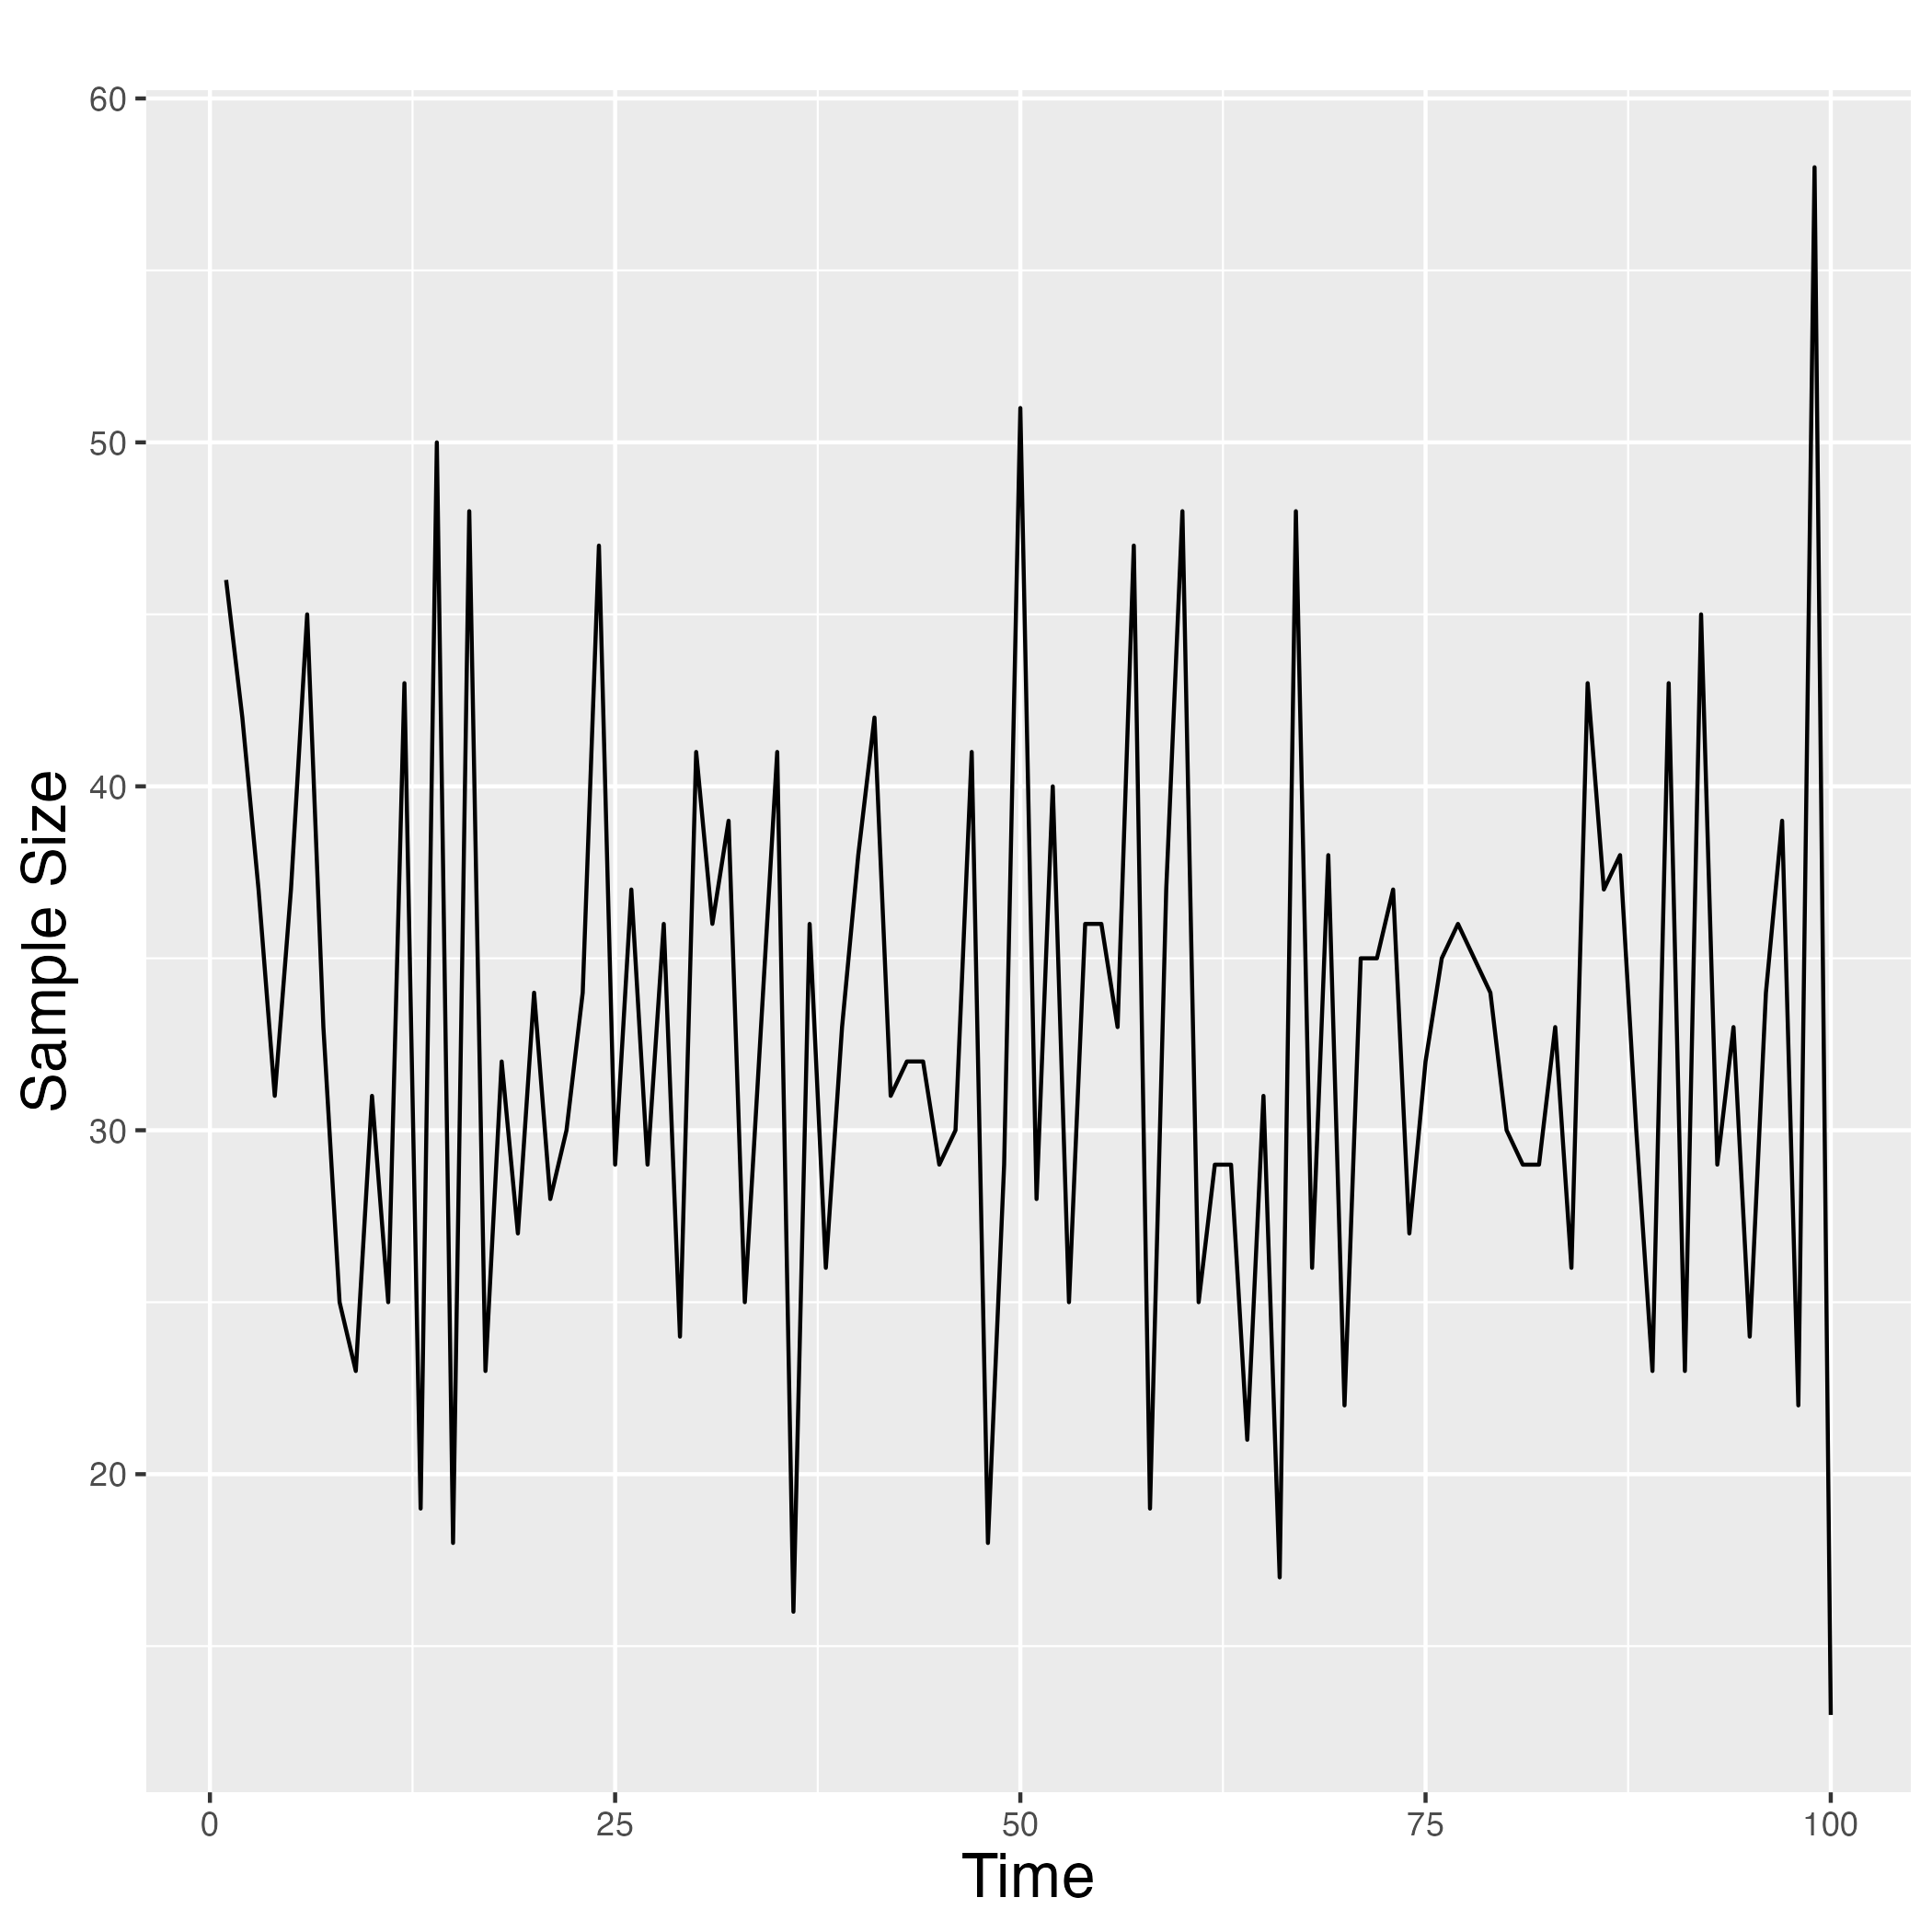
\includegraphics[width=\linewidth]{images/output/inar.png}
        \caption{Sample INAR process}

    \end{subfigure}
    \hfill
    \begin{subfigure}{0.45\textwidth}
        \centering
        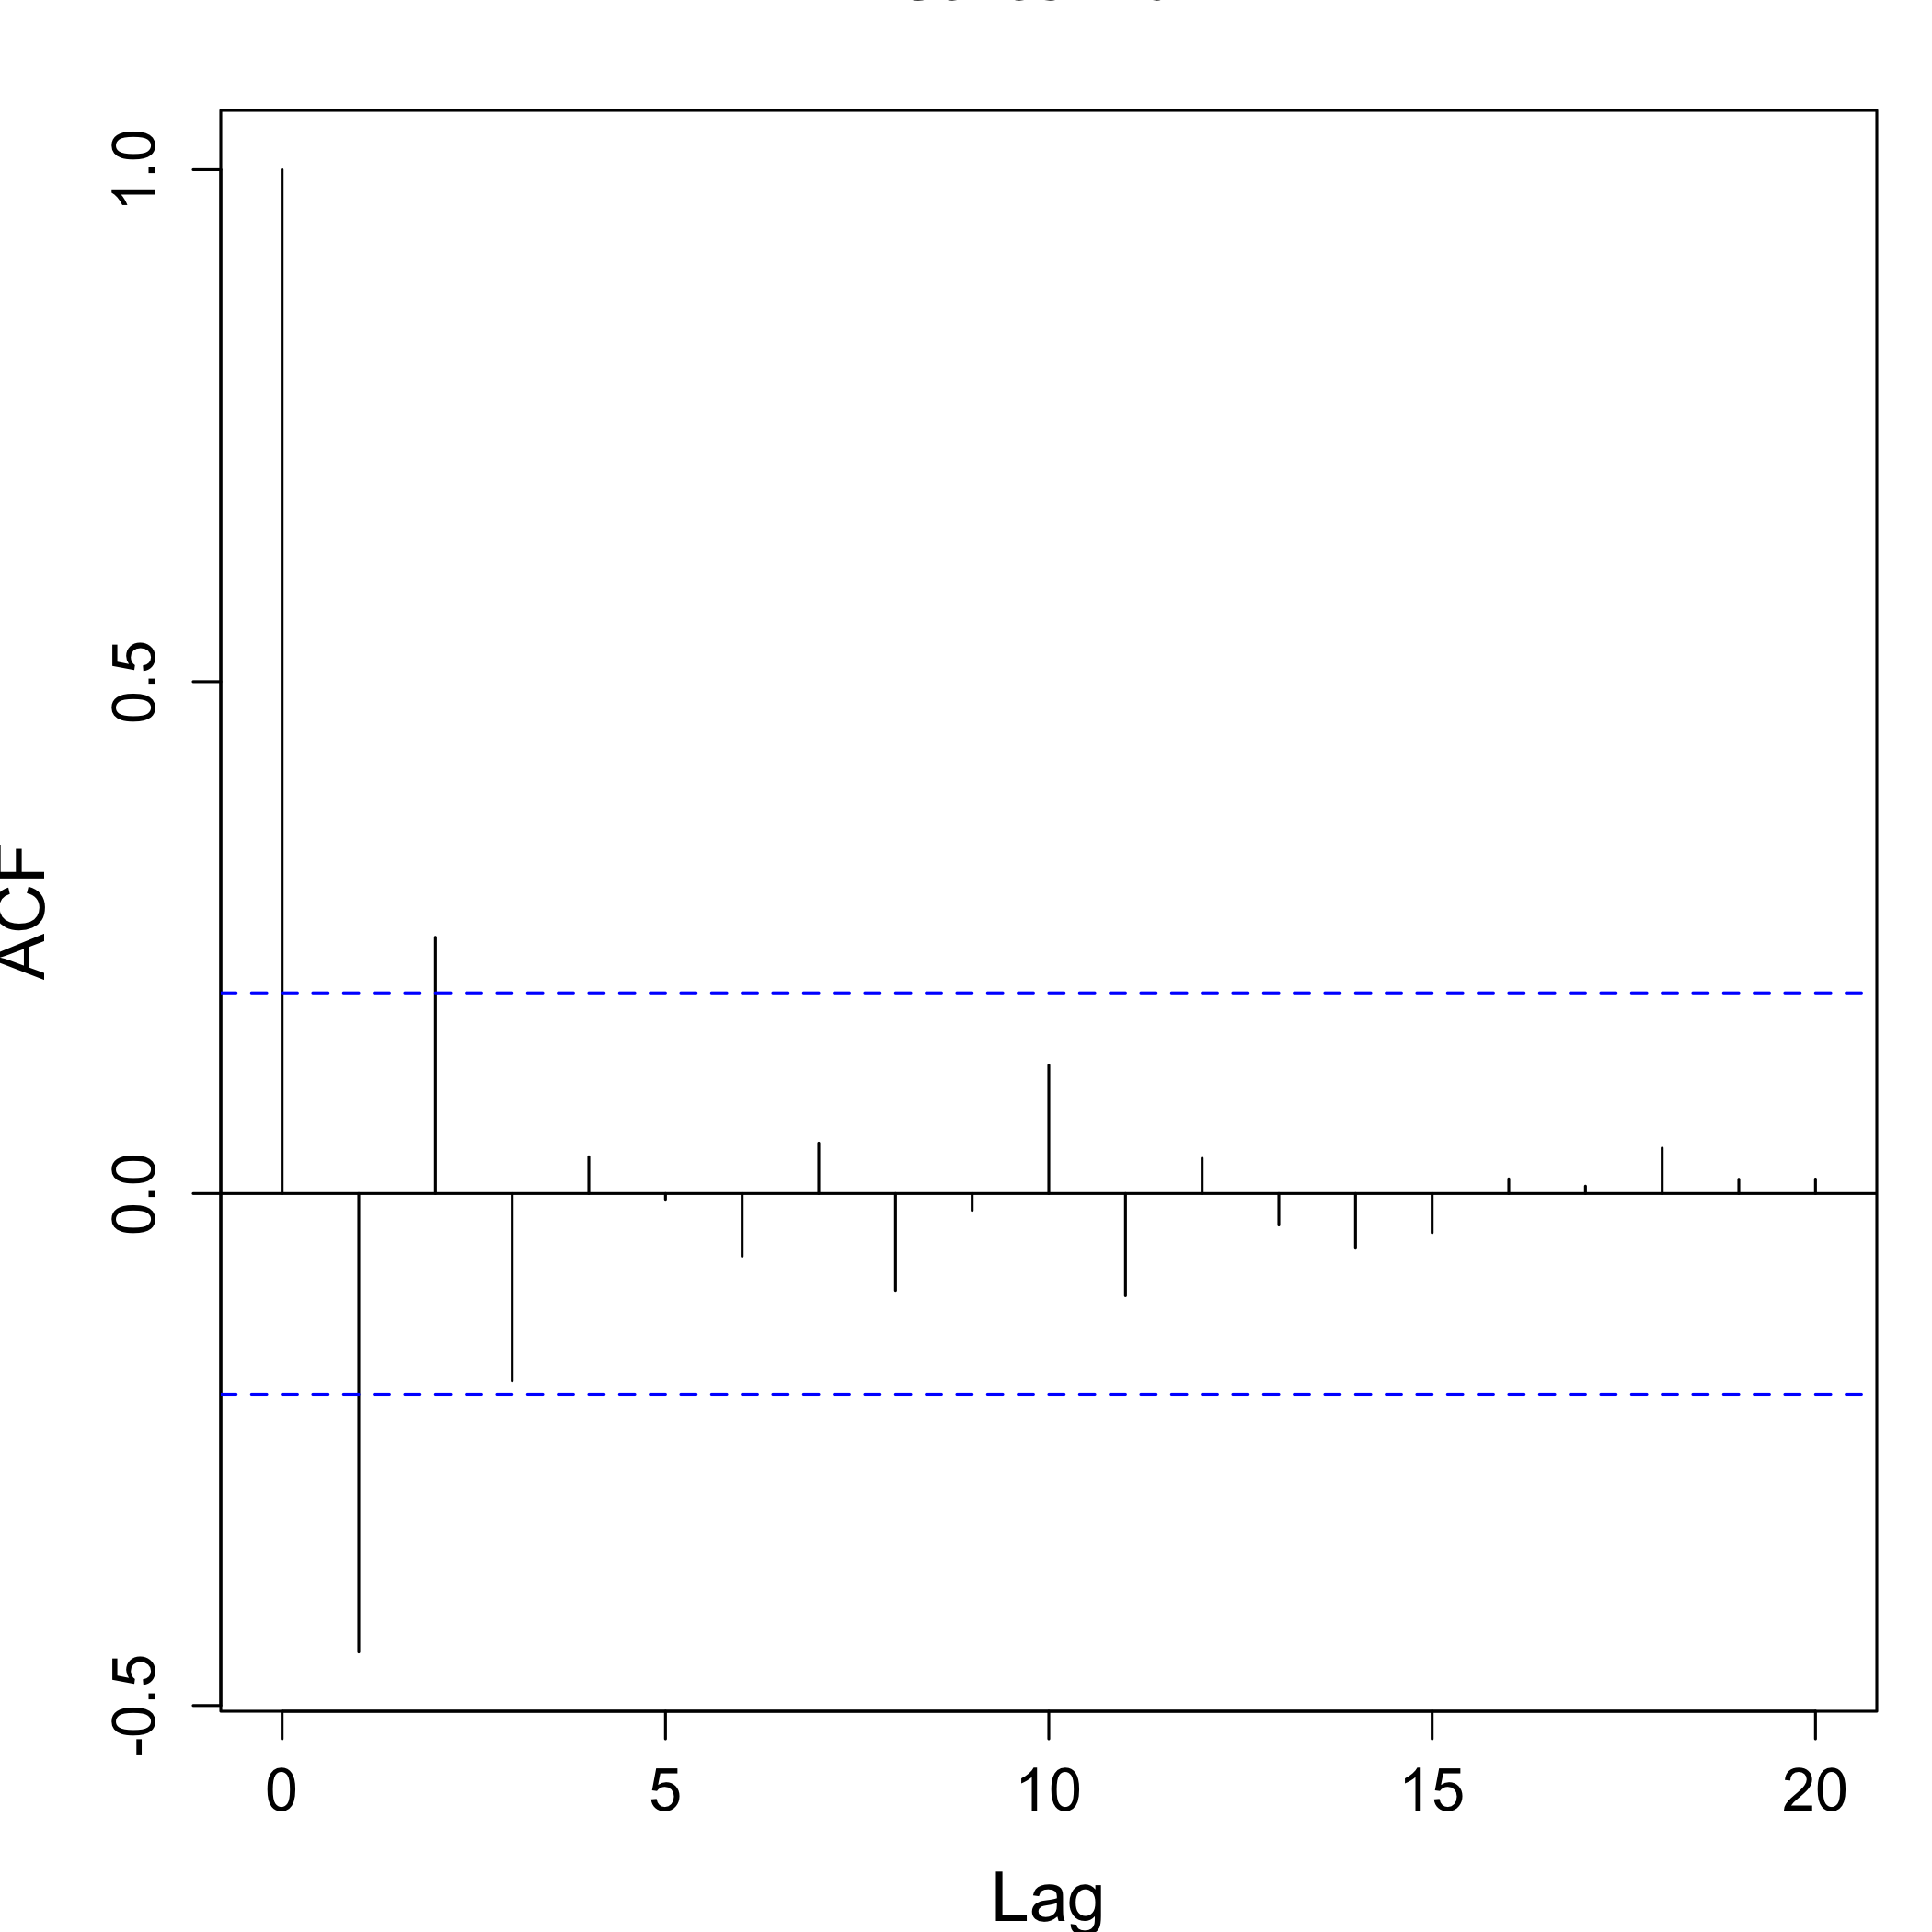
\includegraphics[width=\linewidth]{images/output/inar_acf.png}
        \caption{Corresponding Sample ACF}

    \end{subfigure}
    \caption{A realization of an INAR(2) process with parameters $\alpha = 0.3$, $\beta = 0.8$, $\lambda = 50$}
    \label{fig:inar}
\end{figure}

Such a distribution is strictly stationary and has a constant reciprocal expectation. Were we to loosen the condition of strict stationarity to include \emph{weakly} stationary processes, it cannot be guaranteed that $\{A_t\}$ is white noise. To illustrate this, let's define the random variables $X_\text{odd}$ and $X_\text{even}$:



Thus defined, $X_\text{odd}$ and $X_\text{even}$ have the same first and second moments, $\mathbb{E}(X_\text{odd}) = \mathbb{E}(X_\text{even}) = 2$ and $\mathbb{E}(X_\text{odd}^2) = \mathbb{E}(X_\text{even}^2) = 5$. The time series $\{N_t\}$ defined as equal in distribution to $X_\text{odd}$ for odd values of $t$ and $X_\text{even}$ for even ones is therefore weakly stationary. However, $X_\text{odd}$ and $X_\text{even}$ have different $(-1)^\text{st}$ moments:

$$ \mathbb{E}(X_\text{odd}^{-1}) = \frac{2}{3}\qquad \mathbb{E}(\text{even}^{-1}) = \frac{11}{18} $$

With $N_t$ defined as above, the daily average $A_t$, while independent, has differing variance at odd and even time steps, precluding it from being white noise. It therefore becomes clear that it is not so much independence in sample sizes so much as strict stationarity that ensures $\{A_t\}$ is white noise.


We therefore can extend the procedure outlined by \citep{WongMiller1990} to allow for varying sample size, so long as $\{N_t\}$ is conceivably a realization of a strictly stationary integer-valued time series. $\hat{\sigma}_a^2$ is calculated using Equation \ref{eq:var_a_n}, and its asymptotic variance estimated with \ref{eq:var_a_n}.

\section{ARMA-Noise Processes with Non-stationary Sample Sizes}

Having now established that strictly positive sample sizes being weakly stationary does not guarantee that resulting aggregates are white noise, prompting us to seek any further generalization that would allow for  deterministic changes in $N_t$, something that would seemingly preclude resulting aggregates from being white noise. For instance, the set of sample sizes determined by $N_t = \mathbbm{1}_{2\mathbb{N}}(t)n_1 + \mathbbm{1}_{2\mathbb{N}-1}(t)n_2$ would immediately result in non-stationary noise. However, so far we have only established that $\mathbb{E}(N_t^{-1})$ needs to be constant across $\{t\}$. Let's then look at a distribution with constant $(-1)^\text{st}$ moment and a deterministic, non-constant mean with a trend:

$$ \Omega(N_t) = \{1,t\} $$

We want to construct the distribution of $N_t$ so that $\mathbb{E}(N_t^{-1}) = c$ $\forall$ $t$
$$ \mathbb{E}(N_t^{-1}) = P(N_t=1) + P(N_t=t)t^{-1} = c $$

Because the cardinality of $\Omega(N_t)$ is two, this expression simplifies to:

$$ \mathbb{E}(N_t^{-1}) = (1-P(N_t=t)) + P(N_t=t)t^{-1} = c $$

Defining $p_t$ to be $P(N_t = t)$, we find:
% $$ \mathbb{E}(N_t^{-1}) = (1 - p_t) + p_t t ^ {-1} = c $$

% $$  (1-p_t)t + p_t = tc $$

% $$  t-tp_t + p_t = tc $$

% $$  p_t(1-t) = t(c-1) $$

$$ p_t = \frac{t(c-1)}{1-t} $$

Since $t \geq 1$ for all $t$, $c$ must be less than or equal to one. We therefore flip the direction of subtraction in the numerator and denominator:

$$ p_t = \frac{t(1-c)}{t-1} $$

We can quickly double check that $\mathbb{E}(N_t^{-1})$ is in fact constant:

$$ \mathbb{E}(N_t^{-1}) = 1-p_t + \frac{p_t}{t} = 1 - \frac{t(1-c)}{t-1} + \frac{1-c}{t-1} $$

$$ \mathbb{E}(N_t^{-1}) = \frac{t-1 - t(1-c) + 1-c}{t-1} $$

$$ \mathbb{E}(N_t^{-1}) = \frac{tc - c}{t-1} = \frac{(t-1)c}{t-1} = c $$

Having now defined the distribution of $N_t$, let's find the expression for its mean.

$$ \mathbb{E}(N_t) = 1-p_t + p_tt = 1 + p_t(t-1) = 1 + \frac{t(1-c)}{t-1}(t-1) = 1 + t(1-c) $$

Since $c\in (0,1)$, so too is $(1-c)$ and we get a positive linear trend for $\mathbb{E}(N_t)$. Having a mean that is linear in time, we clearly do not have a stationary process in our sequence of sample sizes. However, the aggregates of the resulting noise are uncorrelated zero-mean random variables with constant variance, and as a result are still white noise. This is visualized in Figure \ref{fig:linear_mean_n_wn}

\begin{figure}[htbp]
    \centering
    % Row 1
    \begin{subfigure}{0.45\textwidth}
        \centering
        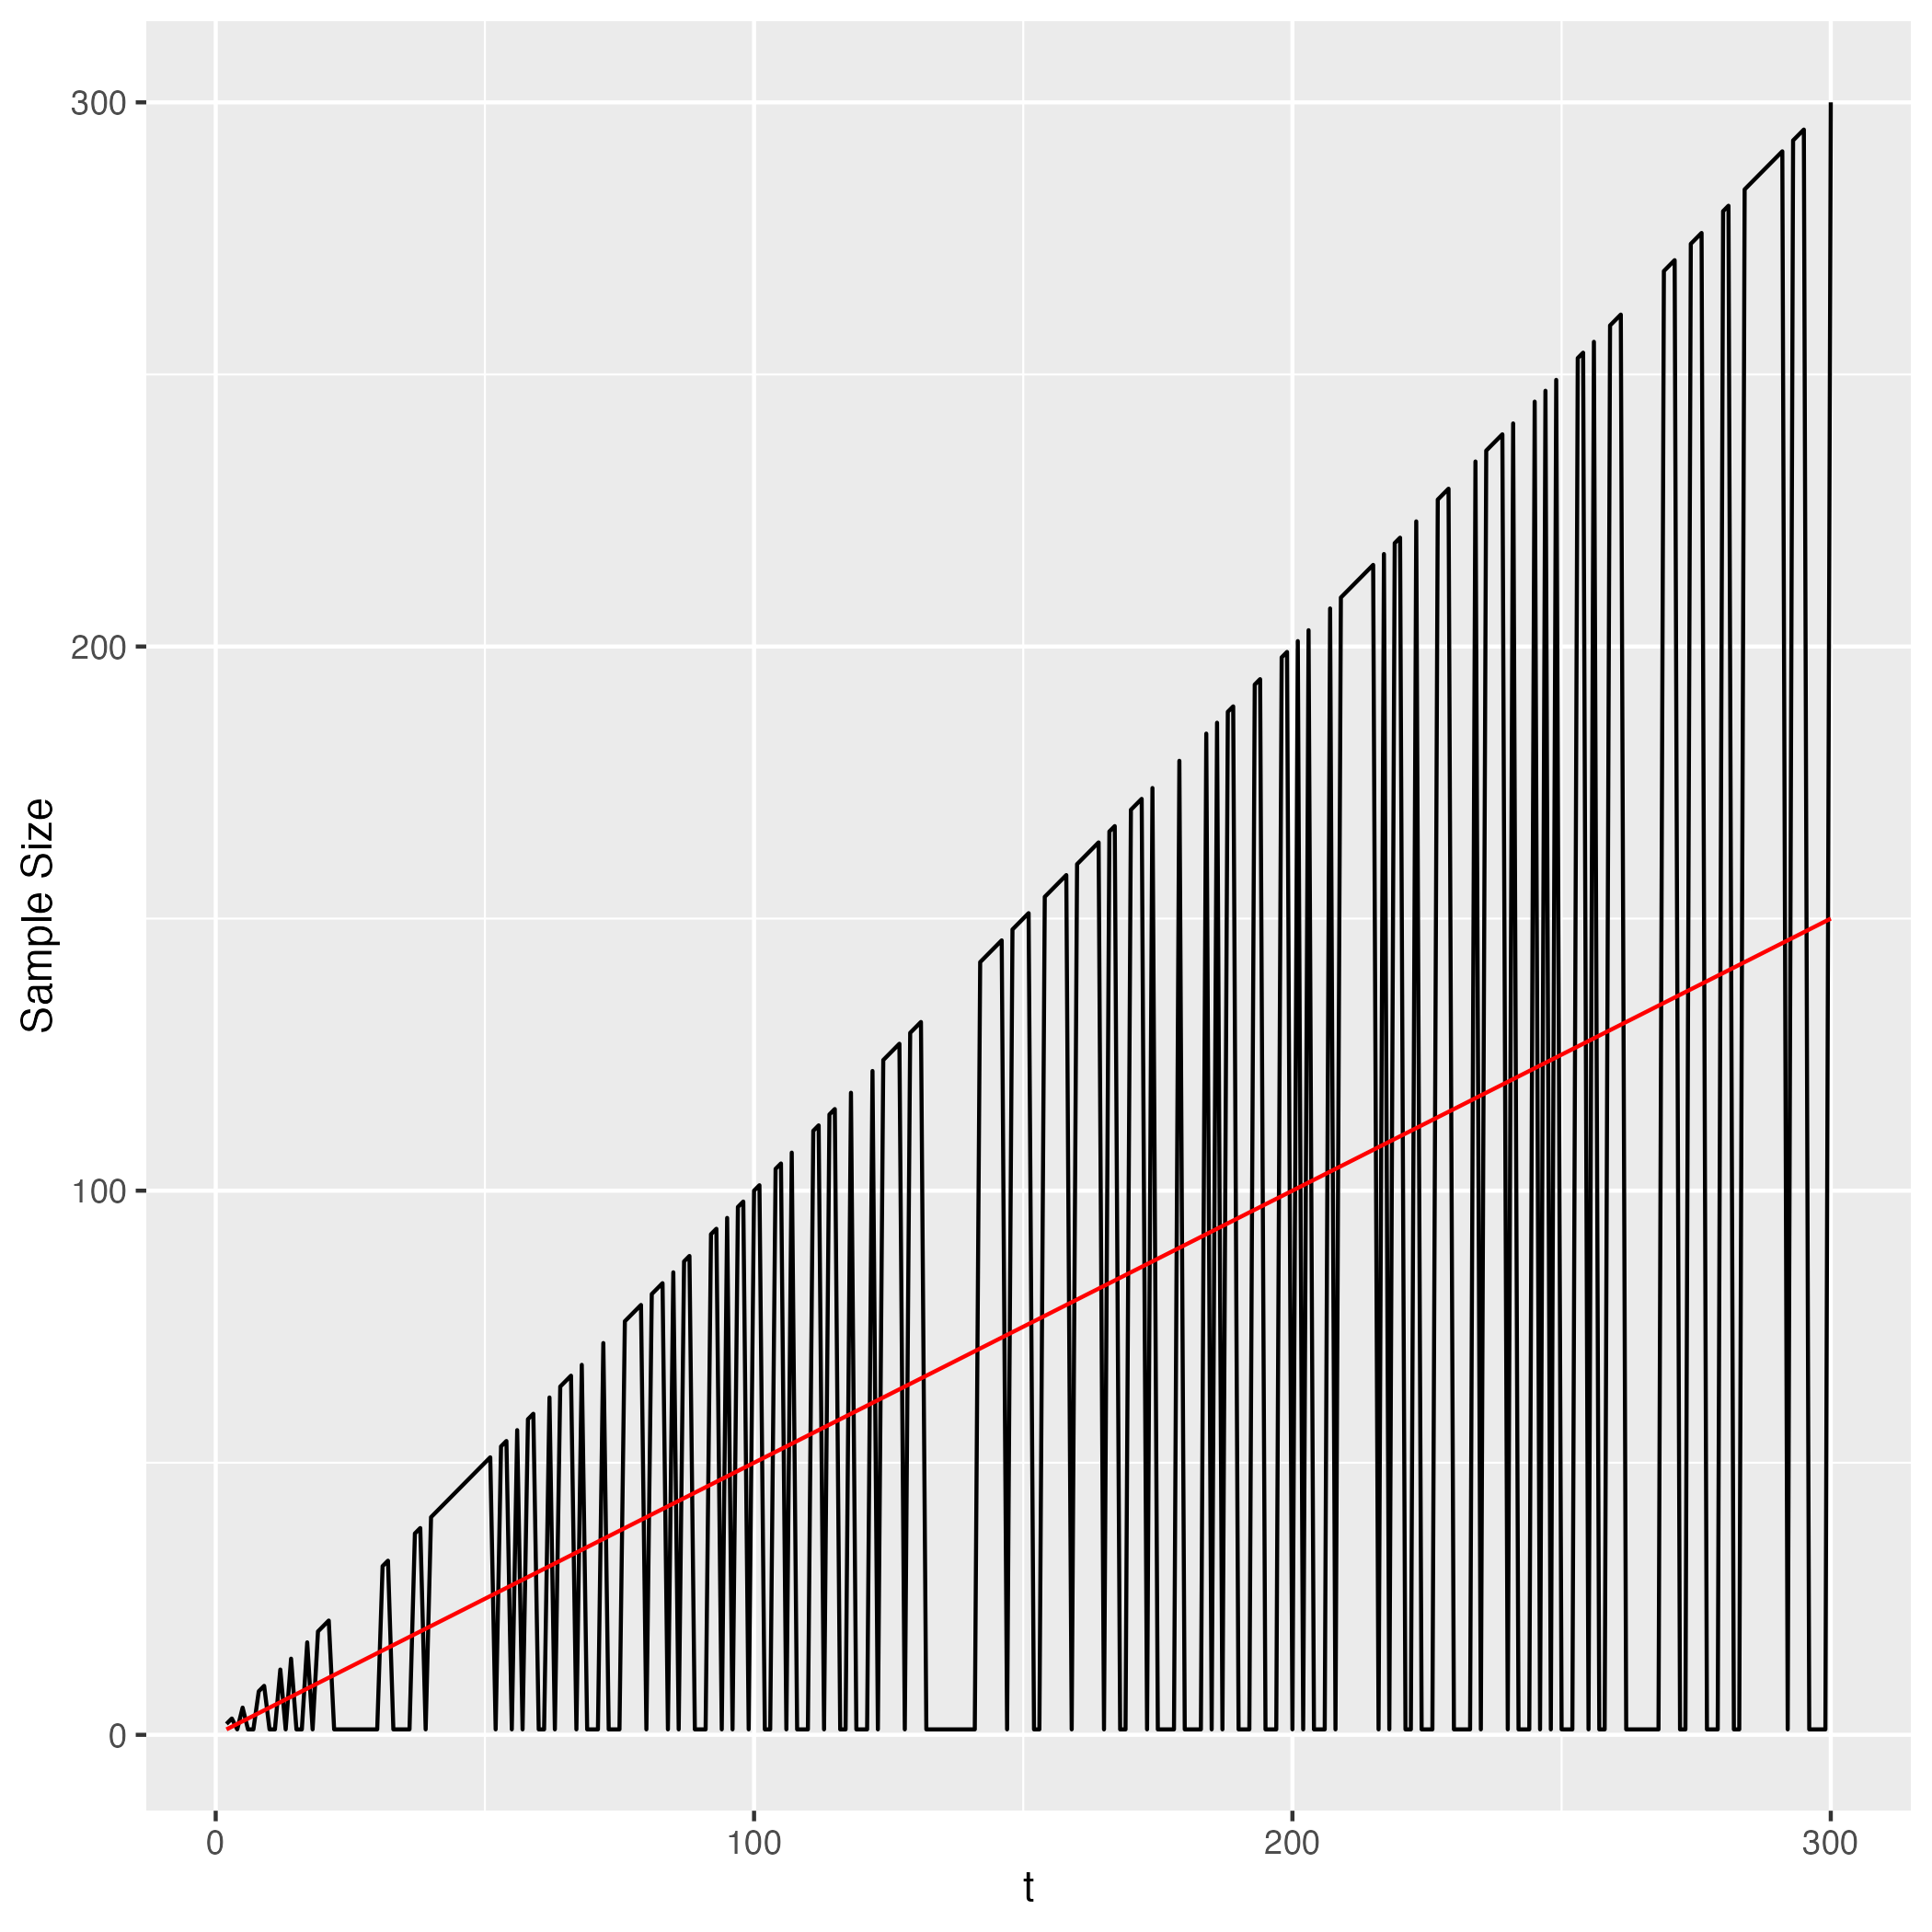
\includegraphics[width=\linewidth]{images/output/constant_inverse_n.png}
        \caption{$\{N_t\}$}
    \end{subfigure}
    \hfill
    \begin{subfigure}{0.45\textwidth}
        \centering
        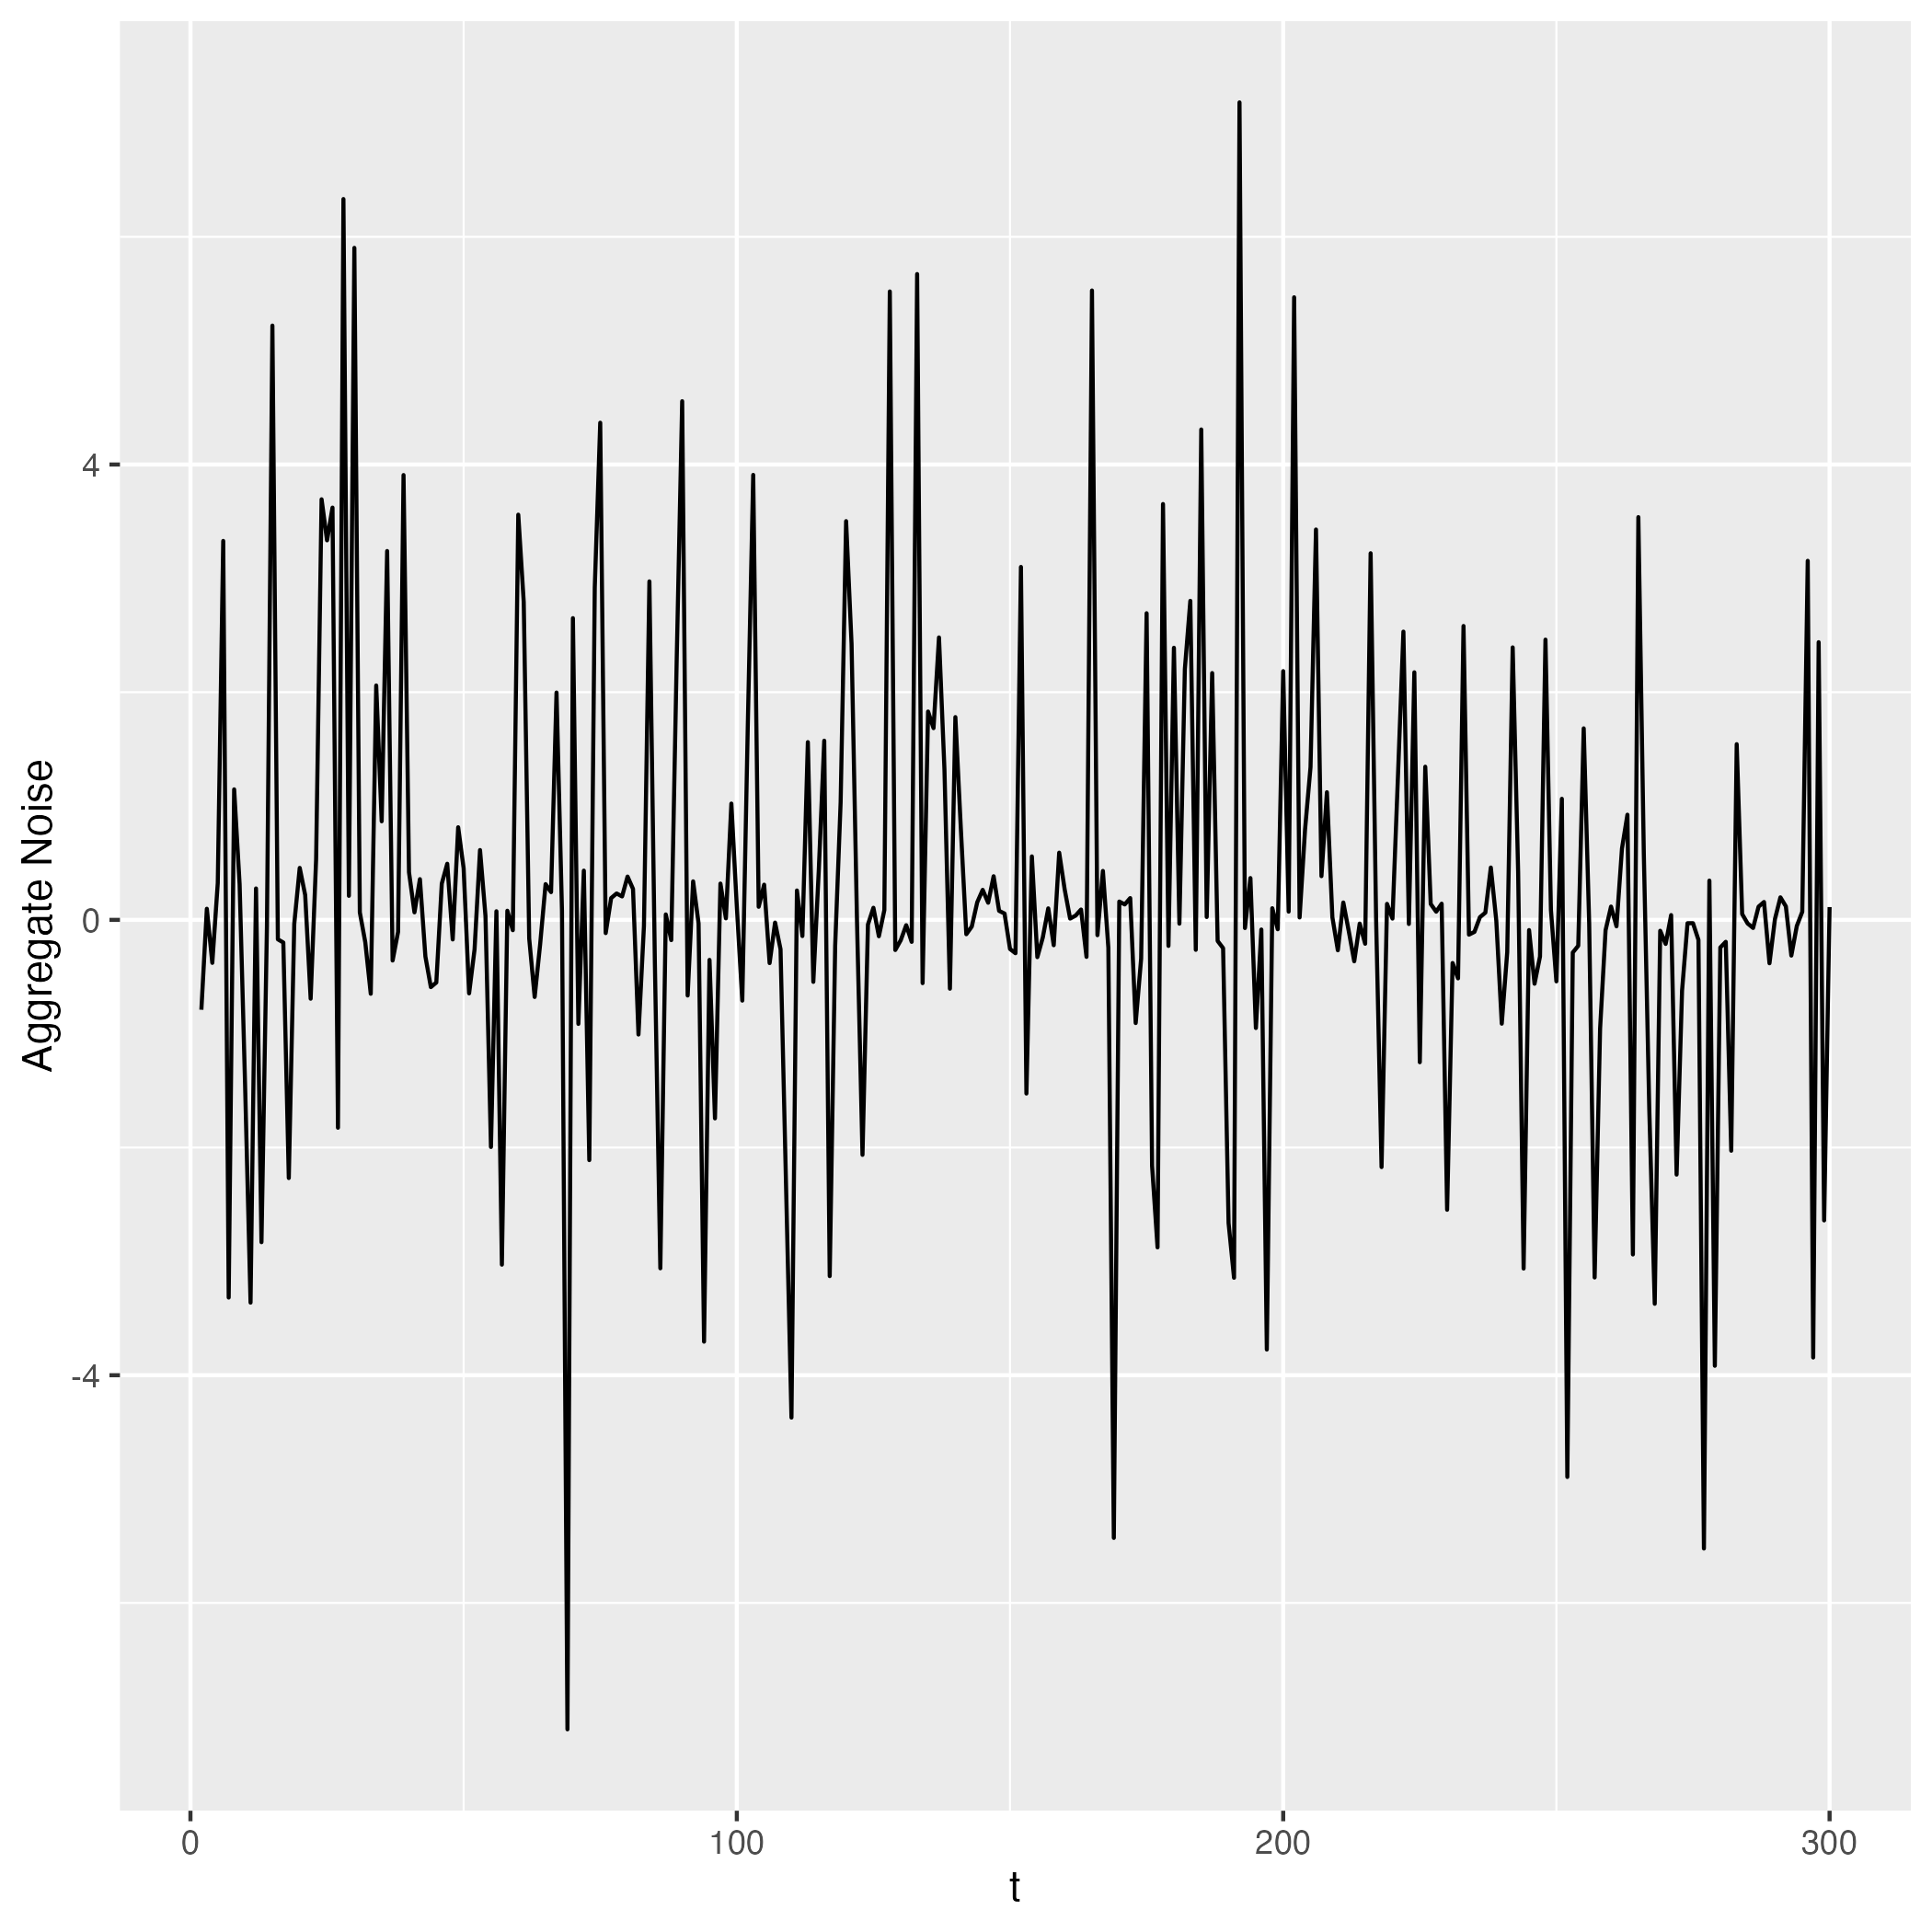
\includegraphics[width=\linewidth]{images/output/constant_inverse_a.png}
        \caption{$\{A_t\}$}
    \end{subfigure}

    \caption{Sample Sizes $\{N_t = (t)M_{t+1} + 1\}$, where $M_t \overset{\text{i.i.d.}}{\sim} \text{Ber}(\frac{t}{2(t-1)})$ and resulting white noise $\{A_t = N_t^{-1}\sum_{i=1}^{N_t}\varepsilon_{ti}\}$ }
    \label{fig:linear_mean_n_wn}
\end{figure}



The takeaway from all this is that a constant expected inverse of $\{N_t\}$ is the critical piece for $\{A_t\}$ to still be white noise.


We distill this observation into the following lemma:


Let $\{\varepsilon_{ti}\}$ be i.i.d. random variables with
\[
\mathbb{E}(\varepsilon_{ti}) = 0, \qquad \mathrm{Var}(\varepsilon_{ti}) = \sigma_\varepsilon^2 < \infty,
\]
independent across both $t$ and $i$. Let $\{N_t\}$ be a stochastic process such that
\[
P(N_t \in \mathbb{N}\setminus\{0\}) = 1 \quad \text{for all } t,
\]
and assume that $\mathbb{E}({N_t^{-1}})$ is constant for all $t$.

Define
\[
A_t := \frac{1}{N_t}\sum_{i=1}^{N_t} \varepsilon_{ti}.
\]

Then $\{A_t\}$ is white noise with $\mathrm{Var}(A_t) = \sigma_\varepsilon^2\,\mathbb{E}(N_t^{-1})$


So long as the set of inverse sample sizes $\{n_t^{-1}\}$ is conceivably of constant expectation, the ARMA-Noise method is applicable.




\medskip




